\chapter{Background}
\label{chap:background}

\section{Background}
Based on the previous work of people using NSGA-II on some multi-objective optimization problems\cite{Magnier_2010_Multiobjective}, we believe we can also applied NSGA-II on our Urban Design Model to find the optimal solution. 

\section{Previous Work}

\subsection{Genetic Algorithm(GA)}
After the Genetic Algorithm was introduced in 1975 by John Henry Holland\cite{Holland_1975_Book}, it has been applied in many areas. With mimicking the process of natural selection, GA uses selection, crossover, and mutation to generate solutions and tries to find the optimal solution for our problems. More specifically, we have an initial population size, then based on our criterion or objective, we give each individual a fitness value. After we select a certain number of individuals from our population based on their fitness, then we apply our crossover function with a crossover probability to have some new offsprings. Next, we apply the mutation function with a mutation probability on the new offsprings. After all those steps, hopefully we can  have a new population which have some better fitness values. Last, we repeat our steps until we achieve our optimal solution.

\subsection{Multiobjective Genetic Algorithm(MOGA)}
When we apply GA to find our optimal solutions, we can divide those problems into two categories based on the number of objectives: Single Objective problems and Multi-Objective problems. Let's take a simple example for single objectives first. For example we want to find the minimum value of \(y=x^2\) with \(x\in [-3,3]\), it is easy to see that we could achieve the minimun value at \(x=0\). When we have two objectives, the problem becomes more complicated. For example we want to minimize both \(y_{1}=x^2\) and \(y_{2}=(x-2)^2\). Then, we are not able to find a specific \(x\) value for this problem. From \autoref{fig:two_functions}, we could see that \(x\) at 0 could give us minimum value of \(y_{1}=x^2\) and \(x\) at 2 could give us minimum value of \(y_{2}=(x-2)^2\). However we are not able to find a \(x\) value which could guarantee us both \(y_{1}\) and \(y_{2}\) at their minimun value. We call \(x=\) \(0\) or \(2\) Pareto Optimal Solutions\cite{Hans_1988_Multicriteria_Pareto_Optimal}\cite{Vira_1983_Multiobjective_Pareto_Optimal}. You could find more information about Pareto Optimal Solutions at our latter sections. Other than \(x=\) \(0\) or \(2\), any points between \(0\) and \(2\) could be a valid compromise solution. 

\begin{figure}[htp] 
\centering
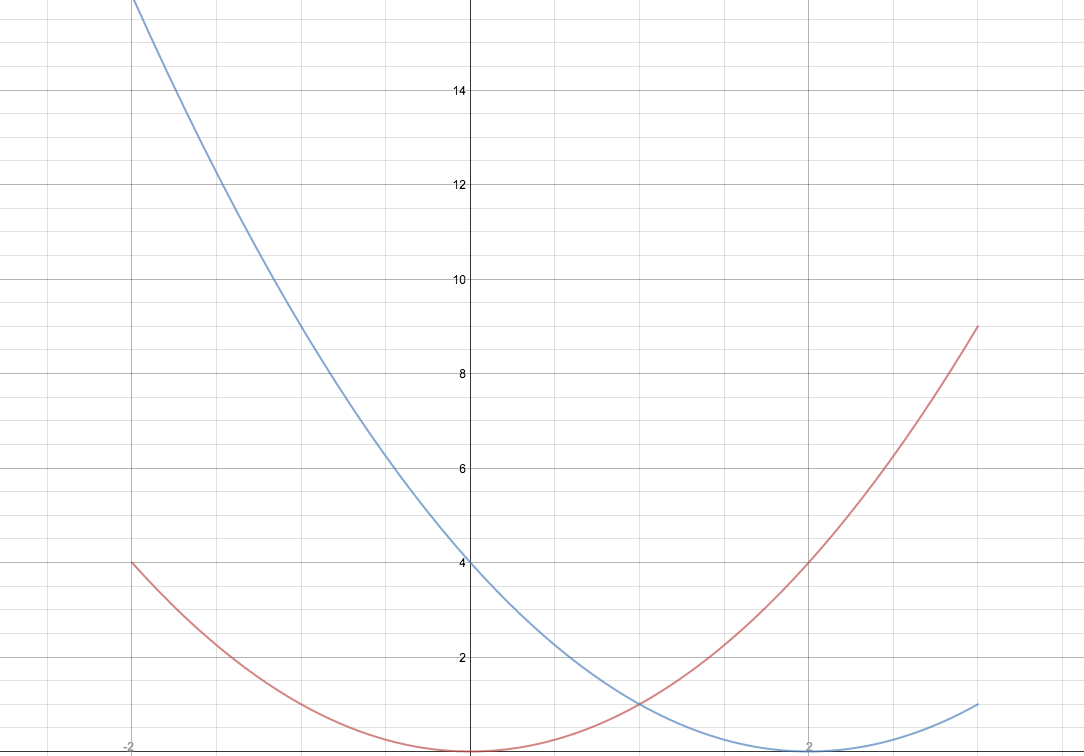
\includegraphics[scale=.2]{images/Figure_1.png}
\caption{Functions \(y_{1}=x^2\) and \(y_{2}=(x-2)^2\)}
\label{fig:two_functions}
\end{figure}

In the real word, there are many kinds of simultaneous optimization of multiple objectives problems. People have tried many methods to find Pareto Optimal Solution. The classical method is to convert multiobjective problem to a single objective problem. In paper \cite{NSGA_1994}, three classical methods are introduced: 1. Objective Weighting, 2. Distance Functions, and 3. Min-Max Formulation. All those methods have one common drawback: it can only give us a single-point solution. However, when decision makers make decision, they often need different alternatives. Another significant drawback of those method is they heavily depend on what weight vector or demand level we choose. So those methods are not efficiency and we probably need to try many times to get a acceptable solution.

Since classical methods to solve multiobjective optimization problems are inadequate and inconvenient, people start to find other ways to implement GA. Next, we will briefly introduce some of those implementations.

\subsection{Vector Evaluated Genetic Algorithm(VEGA)}
VEGA is the first practical algorithm and was developed by Schaffer in 1984\cite{Schaffer_1984_Some}. Instead of changing multiple objective problem to single objective problem, Schaffer modified the simple tripartite genetic algorithm by performing independent selection cycles according to each objective.

\subsection{Nondominated Sorting Genetic Algorithm(NSGA)}

\subsection{Nondominated Sorting Genetic Algorithm II(NSGA-II)}
NSGA-II\cite{NSGA-II} is a very famous multi-objective optimization algorithm which is wide used  to find the optimal solution nowadays. Compare with the previous NSGA, NSGA-II has improved the computational efficiency, elitism, and sharing parameter. For computational complexity of nondominated sorting, it improve from \(O(MN^{3})\) to \(O(MN^{2})\). With the elitism, NSGA-II could not only speed up the GA performance, but also prevent loss of good solutions. Moreover, NSGA II does not need to specify a sharing parameter \(\sigma_{share}\), which is a requirement for pervious multi-objective evolutionary algorithms.

\subsection{Pareto Optimal Solution}

